\documentclass{article}
% -----PACKAGES
%\usepackage[shortend,titlenumbered]{algorithm2e}
%\usepackage{algorithmic}
%\usepackage[plain]{algorithm}
\usepackage{multicol}
\usepackage{color}
\usepackage{multirow}
\usepackage{fancybox}
%\usepackage{index}
\usepackage{varioref}
\usepackage{psfrag}
\usepackage{epsfig}
\usepackage{boxedminipage}
\usepackage{graphicx}
\usepackage{rotating}
\usepackage{amsmath}
\usepackage{amssymb}
%\usepackage{amsfont}
\usepackage{latexsym}
\usepackage{alltt}
%\usepackage[small,bf]{caption}
\usepackage{url}
%\usepackage{citesort}
%\usepackage{crop}
\usepackage{array}
\usepackage{subfigure}
\usepackage{dcolumn}

% -----SETLENGTH
%\setlength{\captionmargin}{20pt} 

% -----NEWCOMMANDS
\newcommand{\nc}{\newcommand}
\nc{\mathsm}[1]{\text{\small{$#1$}}}
\nc{\ubar}[1]{\underset{-}{#1}}
\nc{\optype}{\textrm}
\nc{\EQ}[1]{(\ref{eq:#1})}
\nc{\TAB}[1]{\ref{tab:#1}}
\nc{\FIG}[1]{\ref{fig:#1}}
\nc{\SEC}[1]{\ref{sec:#1}}
\nc{\ALG}[1]{\ref{alg:#1}}
\nc{\CHAP}[1]{\ref{chap:#1}}
\nc{\mtrx}[1]{\boldsymbol{\mathbf{#1}}}
\nc{\vctr}[1]{\boldsymbol{\mathbf{#1}}}
\nc{\grad}{\mbox{\boldmath$\nabla$}}
\nc{\gradient}{\textsl{grad}\,}
\nc{\hessian}{\textsl{grad\,}^2}
\nc{\ii}{\iota}
\nc{\dd}{d}
\nc{\ee}{\mathrm{e}}
\nc{\pdiv}[2]{\partial{#1}/\partial{#2}}
\nc{\dpdiv}[2]{\displaystyle{\frac{\partial{#1}}{\partial{#2}}}}
\nc{\ddiv}[2]{\displaystyle{\frac{\dd{#1}}{\dd{#2}}}}
\nc{\inpr}{\hspace{-1pt}\cdot\hspace{-1pt}}
\nc{\IR}{\mathbb{R}}
\nc{\IN}{\mathbb{N}}
\nc{\IZ}{\mathbb{Z}}
\nc{\IC}{\mathbb{C}}
\nc{\half}{\frac{1}{2}}
\nc{\shalf}{\scriptstyle{\half}} 
\nc{\ds}[1]{\displaystyle{#1}}
\nc{\ts}[1]{\textstyle{#1}}
\nc{\sign}{\optype{sign}}
\nc{\spr}{\optype{spr}}
\nc{\dist}{\optype{dist}}
\nc{\rank}{\optype{rank}}
\nc{\codim}{\optype{codim}}
\nc{\supp}{\optype{supp}}
\nc{\diag}{\optype{diag}}
\nc{\meas}{\optype{meas}}
\nc{\cond}{\optype{cond}}
\nc{\kernel}{\optype{kernel}}
\nc{\spa}{\optype{span}}
\nc{\order}{\mathcal{O}}
\nc{\Fr}{\mathrm{Fr}}
\nc{\Rey}{\mathrm{Re}}
\nc{\Ord}{O}
\nc{\ord}{o}
\nc{\st}{\:{:}\:}
\nc{\closure}[1]{\overline{#1}}
\nc{\emin}[1]{\emph{#1}\index{#1}\/}
\nc{\rmin}[1]{#1\index{{}@{#1}}}
\nc{\Laplace}{\Delta}
\nc{\ie}{i.e.}
\nc{\eg}{e.g.}
%\nc{\union}{\cup}
\nc{\Union}{\bigcup}
\nc{\lf}[1]{\mathsf{#1}}
\nc{\dbar}[1]{\bar{\bar{#1}}}
\nc{\ul}[1]{\underline{#1}}
\nc{\hpt}{\hspace{0.5pt}}
\nc{\E}[1]{\times{}10^{#1}}
\nc{\inp}[2]{\langle{#1},{#2}\rangle}
\nc{\tmpcommand}{}

% -----RENEWCOMMANDS
\renewcommand{\baselinestretch}{1}
\renewcommand{\exp}{\optype{exp}\,}
\renewcommand{\cosh}{\optype{cosh}\,}
\renewcommand{\tanh}{\optype{tanh}\,}
\renewcommand{\sinh}{\optype{sinh}\,}
\renewcommand{\div}[1]{\optype{div}\,{#1}}
\renewcommand{\half}{\mbox{$\frac{1}{2}$}}
%\renewcommand{\descriptionlabel}[1]{\hspace{\labelsep}\emph{#1}}

% -----ETC
\raggedbottom


\DeclareMathOperator{\curl}{\bf curl}
\DeclareMathOperator{\rot}{\rm curl}
\DeclareMathOperator{\divv}{\rm div}
\newcommand{\tro}{\gamma_0}
\newcommand{\trt}{\gamma_{\sft}}
\newcommand{\trn}{\gamma_{\sfn}}

\newcommand{\PT}{{\partial T}}
\newcommand{\bbN}{{\mathbb{N}}}
\newcommand{\bbP}{{\mathbb{P}}}

\newcommand{\scC}{{\mathscr{C}}}
\newcommand{\caD}{{\mathcal{D}}}
\newcommand{\caL}{{\mathcal{L}}}

\newcommand{\sfe}{{\mathsf{e}}}
\newcommand{\sff}{{\mathsf{f}}}
\newcommand{\sft}{{\boldsymbol{\mathsf{t}}}}
\newcommand{\sfn}{{\boldsymbol{\mathsf{n}}}}

%   Common caligraphic abbrevs
\newcommand{\BB}{\mathcal{B}}
\newcommand{\CC}{\mathcal{C}}
\newcommand{\DD}{\mathcal{D}}
\newcommand{\EE}{\mathcal{E}}
\newcommand{\FF}{\mathcal{F}}
\newcommand{\GG}{\mathcal{G}}
\newcommand{\II}{\mathcal{I}}
\newcommand{\JJ}{\mathcal{J}}
\newcommand{\KK}{\mathcal{K}}
\newcommand{\LL}{\mathcal{L}}
\newcommand{\OO}{\mathcal{O}}
\newcommand{\QQ}{\mathcal{Q}}
\newcommand{\RR}{\mathcal{R}}
\newcommand{\TT}{\mathcal{T}}


 %% JAY'S PREAMBLE
 %%========================

%   Math symbol definitions
\def\d{\partial}
%\newsymbol\lee 132E
\newcommand{\union}{\mathop{\bigcup}}
\newcommand{\intersect}{\mathop{\bigcap}}
\newcommand{\binomial}[2]{\ensuremath{
		\begin{pmatrix}{#1}\\{#2}\end{pmatrix}}}
\newcommand{\smallbinomial}[2]{\ensuremath{
		(\begin{smallmatrix}{#1}\\{#2}\end{smallmatrix})}}
\newcommand{\tang}[1]{\ensuremath{{#1}_{\intercal}}} % can use \top
						     % also
\newcommand{\hypergeom}[2]{\ensuremath{\sideset{_{#1}}{_{#2}}{\mathop{F}}}}
%   Difficult names
\newcommand{\Babuska}{Babu{\v{s}}ka}       % Remember: Usage is \Babuska\
\newcommand{\Cea}{C{\'e}a}                 % with trailing `\' to give space
\newcommand{\Poincare}{Poincar{\'{e}}}     % when needed, but when ending
\newcommand{\Nedelec}{N{\'{e}}d{\'{e}}lec} % sentence use \Babuska.
\newcommand{\Frechet}{Fr{\'{e}}chet}
\newcommand{\Muller}{M{\"u}ller}
\newcommand{\LHospital}{L'H{\^{o}}spital}
%   Bold and beautiful
\newcommand{\ba}{{\boldsymbol{a}}}
\newcommand{\bA}{\boldsymbol{A}}
\newcommand{\balpha}{{\boldsymbol{\alpha}}}
\newcommand{\bB}{{\boldsymbol{B}}}
\newcommand{\bb}{{\boldsymbol{b}}}
\newcommand{\bbeta}{{\boldsymbol{\beta}}}
\newcommand{\etab}{{\boldsymbol{\eta}}}
\newcommand{\bC}{{\boldsymbol{C}}}
\newcommand{\bc}{{\boldsymbol{c}}}
\newcommand{\bD}{{\boldsymbol{D}}}
\newcommand{\bd}{{\boldsymbol{d}}}
\newcommand{\db}{{\boldsymbol{\d}}}
\newcommand{\bdelta}{{\boldsymbol{\delta}}}
\newcommand{\bDelta}{{\boldsymbol{\Delta}}}
\newcommand{\beps}{{\boldsymbol{\varepsilon}}}
\newcommand{\be}{{\boldsymbol{e}}}
\newcommand{\bg}{{\boldsymbol{g}}}
\newcommand{\bm}{{\boldsymbol{m}}}
\newcommand{\bn}{{\boldsymbol{n}}}
\newcommand{\bN}{{\boldsymbol{N}}}
\newcommand{\bp}{{\boldsymbol{p}}}
\newcommand{\bpsi}{{\boldsymbol{\psi}}}
\newcommand{\bq}{{\boldsymbol{q}}}
\newcommand{\bxi}{{\boldsymbol{\xi}}}
\newcommand{\bE}{{\boldsymbol{E}}}
\newcommand{\bF}{{\boldsymbol{F}}}
\newcommand{\bh}{{\boldsymbol{h}}}
\newcommand{\bH}{{\boldsymbol{H}}}
\newcommand{\bI}{{\boldsymbol{I}}}
\newcommand{\bj}{{\boldsymbol{j}}}
\newcommand{\bJ}{{\boldsymbol{J}}}
\newcommand{\bK}{{\boldsymbol{K}}}
\newcommand{\bk}{{\boldsymbol{k}}}
\newcommand{\bll}{{\boldsymbol{\ell}}}
\newcommand{\bL}{{\boldsymbol{L}}}
\newcommand{\blambda}{{\boldsymbol{\lambda}}}
\newcommand{\bmu}{{\boldsymbol{\mu}}}
\newcommand{\bM}{{\boldsymbol{M}}}
\newcommand{\bomega}{{\boldsymbol{\omega}}}
\newcommand{\bP}{{\boldsymbol{P}}}
\newcommand{\bphi}{{\boldsymbol{\phi}}}
\newcommand{\bQ}{{\boldsymbol{Q}}}
\newcommand{\bG}{{\boldsymbol{G}}}
\newcommand{\bu}{{\boldsymbol{u}}}
\newcommand{\bU}{{\boldsymbol{U}}}
\newcommand{\bV}{{\boldsymbol{V}}}
\newcommand{\bX}{{\boldsymbol{X}}}
\newcommand{\bv}{{\boldsymbol{v}}}
\newcommand{\bw}{{\boldsymbol{w}}}
\newcommand{\bW}{{\boldsymbol{W}}}
\newcommand{\bR}{{\boldsymbol{R}}}
\newcommand{\br}{{\boldsymbol{r}}}
\newcommand{\bS}{{\boldsymbol{S}}}
\newcommand{\bT}{{\boldsymbol{T}}}
\newcommand{\btau}{{\boldsymbol{\tau}}}
\newcommand{\bt}{{\boldsymbol{t}}}
\newcommand{\bx}{{\boldsymbol{x}}}
\newcommand{\by}{{\boldsymbol{y}}}
\newcommand{\bz}{{\boldsymbol{z}}}
\newcommand{\bzero}{{\boldsymbol{0}}}
\newcommand{\bZ}{{\boldsymbol{Z}}}
%   Common scalar fields
\newcommand{\RRR}{\mathbb{R}}
\newcommand{\CCC}{\mathbb{C}}
\newcommand{\ZZZ}{\mathbb{Z}}
\newcommand{\NNN}{\mathbb{N}}
%   Differential operators
\newcommand{\dive}{\mathop\mathrm{div}}
%\newcommand{\grad}{\ensuremath{\mathop{{\bf{grad}}}}}
%\newcommand{\curl}{{\ensuremath\mathop{\mathbf{curl}\,}}}
\newcommand{\Curl}{ {\bf Curl}}
\newcommand{\dx}{\ensuremath{\mathrm{d}x}}
\newcommand{\dy}{\ensuremath{\mathrm{d}y}}
\newcommand{\dr}{\ensuremath{\mathrm{d}r}}
\newcommand{\dR}{\ensuremath{\mathrm{d}R}}
\newcommand{\drho}{\ensuremath{\mathrm{d}\rho}}
\newcommand{\dz}{\ensuremath{\mathrm{d}z}}
\newcommand{\dzeta}{\ensuremath{\mathrm{d}\zeta}}
%   Wordy math symbols
\newcommand{\card}{\ensuremath{\mathop\mathrm{card}}}
%\newcommand{\diag}{\ensuremath{\mathop\mathrm{diag}}}
\newcommand{\diam}{\ensuremath{\mathop\mathrm{diam}}}
%\newcommand{\dist}{\mathop\mathrm{dist}}
\newcommand{\Ker}{\mathop\mathrm{Ker}}
\newcommand{\Range}{\mathop\mathrm{Range}}
%\newcommand{\rank}{\mathop\mathrm{rank}}
%\newcommand{\meas}{\mathop\mathrm{meas}}
\newcommand{\Forall}{\quad\text{for all }}
%\newcommand{\supp}{\mathop\mathrm{supp}}
\newcommand{\Span}{\mathop\mathrm{Span}}
\newcommand{\Hdiv}[1]{\bH(\dive,#1)}
%\newcommand{\Hcurl}[1]{\bH(\curl,#1)}
%   Common caligraphic abbrevs
%\newcommand{\BB}{\mathcal{B}}
%\newcommand{\CC}{\mathcal{C}}
%\newcommand{\DD}{\mathcal{D}}
%\newcommand{\EE}{\mathcal{E}}
%\newcommand{\FF}{\mathcal{F}}
%\newcommand{\GG}{\mathcal{G}}
%\newcommand{\II}{\mathcal{I}}
%\newcommand{\JJ}{\mathcal{J}}
%\newcommand{\KK}{\mathcal{K}}
%\newcommand{\LL}{\mathcal{L}}
%\newcommand{\OO}{\mathcal{O}}
%\newcommand{\QQ}{\mathcal{Q}}
%\newcommand{\RR}{\mathcal{R}}
%\newcommand{\TT}{\mathcal{T}}
%   Variations on standard symbols
\newcommand{\veps}{\varepsilon}
\newcommand{\vlam}{\varLambda}
\newcommand{\vpi}{\varPi}
\newcommand{\vPi}{\boldsymbol{\varPi}}
\newcommand{\vsig}{\varSigma}
\newcommand{\vbt}{\boldsymbol{\varTheta}}
\newcommand{\vPsi}{\boldsymbol{\varPsi}}
%\newcommand{\ii}{\hat{\imath}}
%   Innerproducts, norms, etc
\newcommand{\ntrip}[1]{|\!|\!| {#1} |\!|\!|}
\newcommand{\ip}[1]{\langle {#1} \rangle}
%   Utilities
\newcommand{\blnk}{\underline{\hspace{3cm}}\;}
\newcommand{\marg}[1]{\marginpar{\tiny{\framebox{\parbox{1.7cm}{#1}}}}}
\newcommand{\degreeC}[1]{\ensuremath{{#1\,}^\circ\!\text{C}}}
                        % try also  \textcelsius of textcomp package
%   Trademarked names \texttrademark, \textregistered
\newcommand{\matlab}{MATLAB\textregistered\renewcommand{\matlab}{MATLAB}}
\newcommand{\femlab}{FEMLAB\textregistered\renewcommand{\femlab}{FEMLAB}}

%   Style preferences
\renewcommand{\thefootnote}{\fnsymbol{footnote}} % Use symbols instead of
						 % numbers for footnotes
						 

\newcommand{\Eg}{\EE^\mathrm{grad}}
\newcommand{\Ec}{\boldsymbol{\EE}^\mathrm{curl}}
\newcommand{\Ed}{\boldsymbol{\EE}^\mathrm{div}}


\newcommand{\bfdu}{\mbox{\boldmath $\delta u$}}
\newcommand{\bfdv}{\mbox{\boldmath $\delta v$}}
\newcommand{\du}{{\delta u}}
\newcommand{\dv}{{\delta v}}
\newcommand{\bfnabt}{\widetilde{\bfnab}}
\newcommand{\bfepst}{\widetilde{\bfeps}}

\usepackage{pgf,tikz}
\usetikzlibrary{arrows}

\author{Truman E. Ellis}
\title{Notes on Space-Time for the Heat Equation}

\begin{document}
\maketitle

\section*{Introduction}
For the following discussion, let (master) element $K$ be a tensor product of a spatial
component, $X$, and a time component, $T$. Let $\Grad$ denote the spatial
gradient, and $\frac{\partial}{\partial t}$ denote the time derivative.
Let $\mathbf{n}=(\mathbf{n_x},n_t)^T$ be the full space-time normal vector
where $\mathbf{n_x}$ is the spatial component and $n_t$ is the temporal
component.

We make a few assumptions about the space-time mesh. Figures \ref{fig:mesh1}
and \ref{fig:mesh2} represent two possible temporal refinements of the center
element. We will see later in the discussion that flux variables $\hat f$ are
not well defined on constant-time interfaces, while trace variables are
defined on all element interfaces. Mathematically, the mesh in
Figure~\ref{fig:mesh2} is perfectly valid, but for practical reasons we think
it would be best to avoid these kinds of temporal refinements. For one, we
would have to add logic that adds new flux variables if the new element
division does not follow a constant-time contour. Also, the new flux variable
becomes ill-defined as the interface approaches ``horizontal''. Of course,
this assumption of only making constant-time temporal refinements doesn't
guarantee that the won't run into this ``near-horizontal'' condition, but if
``top'' and ``bottom'' faces are guaranteed to be ``horizontal'' then mesh
quality guidelines should make such situations undesirable for other reasons.
We can do some
experiments with the current code to approximate how catastrophic this
``near-horizontal'' refinement would be. This is analogous to pure convection
when the convection vector aligns (or nearly aligns) with the mesh. In which
case, the cross-stream flux degenerates. This is something I'll be looking
into soon.

\begin{figure}[p]
\begin{tikzpicture}[line cap=round,line join=round,>=triangle 45,x=2.0cm,y=2.0cm]
\clip(-0.7,-1.01) rectangle (5.27,2.29);
\draw (0,2)-- (0,0);
\draw (0,0)-- (1,0);
\draw (1,0)-- (4,0);
\draw (4,0)-- (5,0);
\draw (5,0)-- (5,2);
\draw (5,2)-- (3,2);
\draw (3,2)-- (2,2);
\draw (2,2)-- (0,2);
\draw (1,0)-- (1.5,1);
\draw (1.5,1)-- (2,2);
\draw (1.5,1)-- (3.5,1);
\draw (3,2)-- (3.5,1);
\draw (3.5,1)-- (4,0);
\draw (-0.21,1.26) node[anchor=north west] {$\hat f$};
\draw (4.82,1.19) node[anchor=north west] {$\hat f$};
\draw (3.42,0.75) node[anchor=north west] {$\hat f$};
\draw (1.1,0.78) node[anchor=north west] {$\hat f$};
\draw (1.56,1.68) node[anchor=north west] {$\hat f$};
\draw (2.99,1.68) node[anchor=north west] {$\hat f$};
\draw (0.05,1.23) node[anchor=north west] {$\hat u$};
\draw (1.45,0.76) node[anchor=north west] {$\hat u$};
\draw (3.79,0.74) node[anchor=north west] {$\hat u$};
\draw (2.47,1.3) node[anchor=north west] {$\hat u$};
\draw (3.33,1.66) node[anchor=north west] {$\hat u$};
\draw (1.89,1.65) node[anchor=north west] {$\hat u$};
\draw (5.07,1.18) node[anchor=north west] {$\hat u$};
\draw (4.44,0.29) node[anchor=north west] {$\hat u$};
\draw (2.46,0.29) node[anchor=north west] {$\hat u$};
\draw (0.45,0.29) node[anchor=north west] {$\hat u$};
\draw (2.44,2.04) node[anchor=north west] {$\hat u$};
\draw (0.76,1.99) node[anchor=north west] {$\hat u$};
\draw (4.21,2) node[anchor=north west] {$\hat u$};
\draw [->] (-0.5,-0.5) -- (-0.5,0);
\draw [->] (-0.5,-0.5) -- (0,-0.5);
\draw (-0.54,0.29) node[anchor=north west] {$t$};
\draw (0.07,-0.35) node[anchor=north west] {$x$};
\end{tikzpicture}
\caption{Allowable refinement pattern illustrating support of trace and flux
variables}
\label{fig:mesh1}
\end{figure}

\begin{figure}[p]
\begin{tikzpicture}[line cap=round,line join=round,>=triangle 45,x=2.0cm,y=2.0cm]
\clip(-0.7,-1.09) rectangle (5.27,2.29);
\draw (0,2)-- (0,0);
\draw (0,0)-- (1,0);
\draw (1,0)-- (4,0);
\draw (4,0)-- (5,0);
\draw (5,0)-- (5,2);
\draw (5,2)-- (3,2);
\draw (3,2)-- (2,2);
\draw (2,2)-- (0,2);
\draw (1,0)-- (1.2,0.4);
\draw (1.2,0.4)-- (2,2);
\draw (1.2,0.4)-- (3.5,1);
\draw (3,2)-- (3.5,1);
\draw (3.5,1)-- (4,0);
\draw (-0.21,1.26) node[anchor=north west] {$\hat f$};
\draw (4.82,1.19) node[anchor=north west] {$\hat f$};
\draw (3.42,0.75) node[anchor=north west] {$\hat f$};
\draw (0.9,0.38) node[anchor=north west] {$\hat f$};
\draw (1.36,1.38) node[anchor=north west] {$\hat f$};
\draw (2.99,1.68) node[anchor=north west] {$\hat f$};
\draw (0.05,1.23) node[anchor=north west] {$\hat u$};
\draw (1.25,0.36) node[anchor=north west] {$\hat u$};
\draw (3.79,0.74) node[anchor=north west] {$\hat u$};
\draw (2.47,1) node[anchor=north west] {$\hat u$};
\draw (3.33,1.66) node[anchor=north west] {$\hat u$};
\draw (1.79,1.35) node[anchor=north west] {$\hat u$};
\draw (5.07,1.18) node[anchor=north west] {$\hat u$};
\draw (4.44,0.29) node[anchor=north west] {$\hat u$};
\draw (2.46,0.29) node[anchor=north west] {$\hat u$};
\draw (0.45,0.29) node[anchor=north west] {$\hat u$};
\draw (2.44,2.04) node[anchor=north west] {$\hat u$};
\draw (0.76,1.99) node[anchor=north west] {$\hat u$};
\draw (4.21,2) node[anchor=north west] {$\hat u$};
\draw [->] (-0.5,-0.5) -- (-0.5,0);
\draw [->] (-0.5,-0.5) -- (0,-0.5);
\draw (-0.54,0.29) node[anchor=north west] {$t$};
\draw (0.07,-0.35) node[anchor=north west] {$x$};
\draw (2.45,0.73) node[anchor=north west] {$\hat f$};
\end{tikzpicture}
\caption{Questionable refinement pattern - as the division approaches
horizontal, $\hat f$ degenerates}
\label{fig:mesh2}
\end{figure}

\section*{Function Spaces}
The heat equation is
\[
\frac{\partial u}{\partial t}-\epsilon\Delta u=f
\]
As a first order system, this is
\begin{align}
  \frac{1}{\epsilon}\bfsigma-\Grad u&=0\\
  \frac{\partial u}{\partial t}-\Div\bfsigma&=f
  \label{eq:firstOrderSystem}
\end{align}
Before we transition to thinking of field, trace, and flux variables, we want
to examine what kind of spaces $u$ and $\bfsigma$ should live in.
From the above formulation we can deduce that
\[
u,\bfsigma,\Grad u,\frac{\partial u}{\partial t}-\Div\bfsigma\in L^2
\]
If we view $\{-\bfsigma,u\}:=\mathbf{U}$ as a group variable, then the last
condition tells us that $\mathbf{U}\in H(\mathrm{div},K)$. In particular, this
means that across a constant-time interface, $u\cdot n_t$ should
be continuous, and across a non-constant-time interface,
$-\bfsigma\cdot\mathbf{n_x}+u\cdot n_t$ should be continuous.

If we take the typical volume-centered, face-centered, edge-centered,
node-centered approach, then we can see that $u$ should have a volume-centered
component, all face-centered components, and edge-centered components on
non-constant-time edges. On the other hand, $\bfsigma$ should have a
volume-centered component and face-centered components on all non-constant
time interfaces.

Now we split $u$ and $\bfsigma$ into field, trace, and flux parts.  It is easy
to see that our new field variable $u$ is a simple scalar valued,
volume-centered $L^2$ variable on each space-time element.  And the field
variable $\bfsigma$ is a vector valued, volume-centered $\mathbf{L}^2$
variable with dimension equal to the spatial dimension. We illustrate the
support in Figure~\ref{fig:field3D} as a blue volume centered box on a 3D
space-time master element.

\begin{figure}[!h]
  \centering
  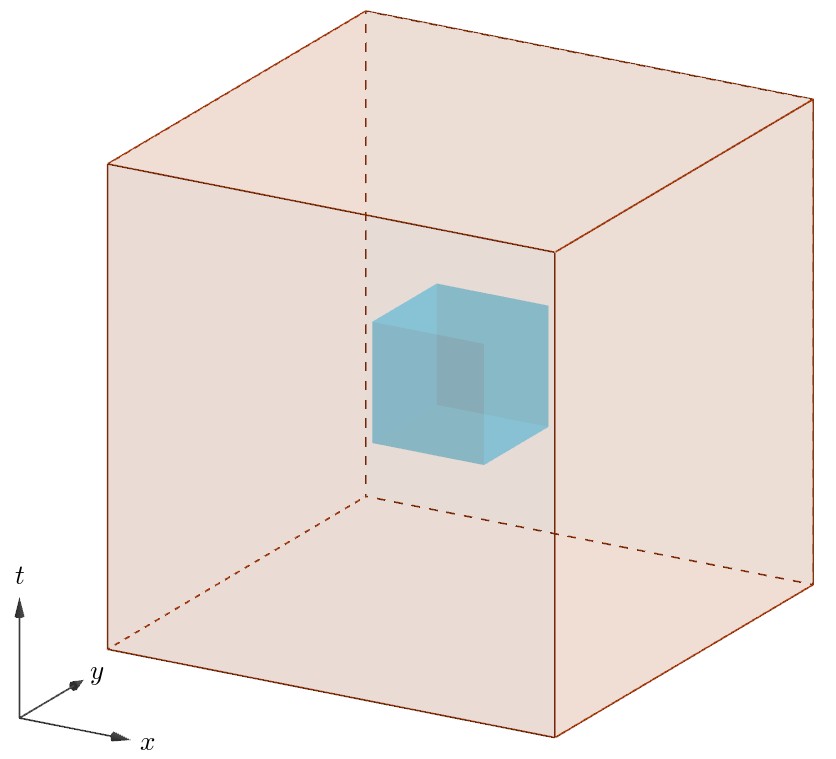
\includegraphics[width=0.7\textwidth]{field3D.png}
  \caption{Support for $u$ and $\bfsigma$}
  \label{fig:field3D}
\end{figure}

Now for the trace and flux variables. $\hat u$ is probably the most
complicated trial variable in the system. It will obviously have face-centered
components on all faces, but it also needs to maintain full continuity in
spatial directions, necessitating the need for edge-centered components on
non-horizontal edges. The face-centered bases have support only on a shared
face between two elements. The edge-centered bases on the other hand have
support on all faces connected to that edge. We illustrate the support in
Figure~\ref{fig:trace3D}. $\hat f$ is much simpler by comparison. It only has
scalar face-centered components on non-horizontal faces. Again, its support is
shown in Figure~\ref{fig:flux3D}.

\begin{figure}[p]
  \centering
  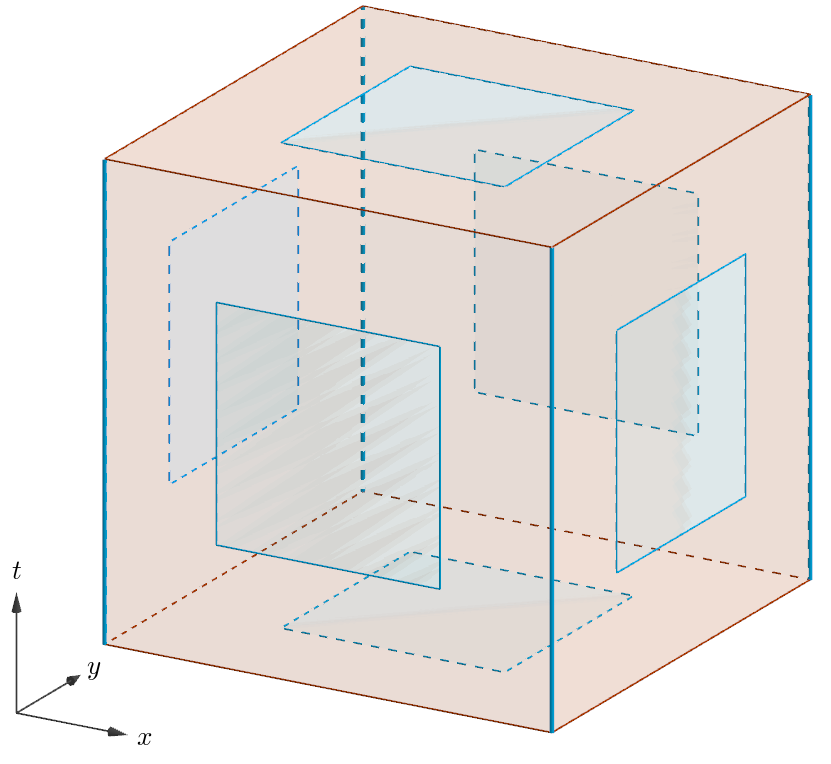
\includegraphics[width=0.7\textwidth]{trace3D.png}
  \caption{Support for $\hat u$}
  \label{fig:trace3D}
\end{figure}

\begin{figure}[p]
  \centering
  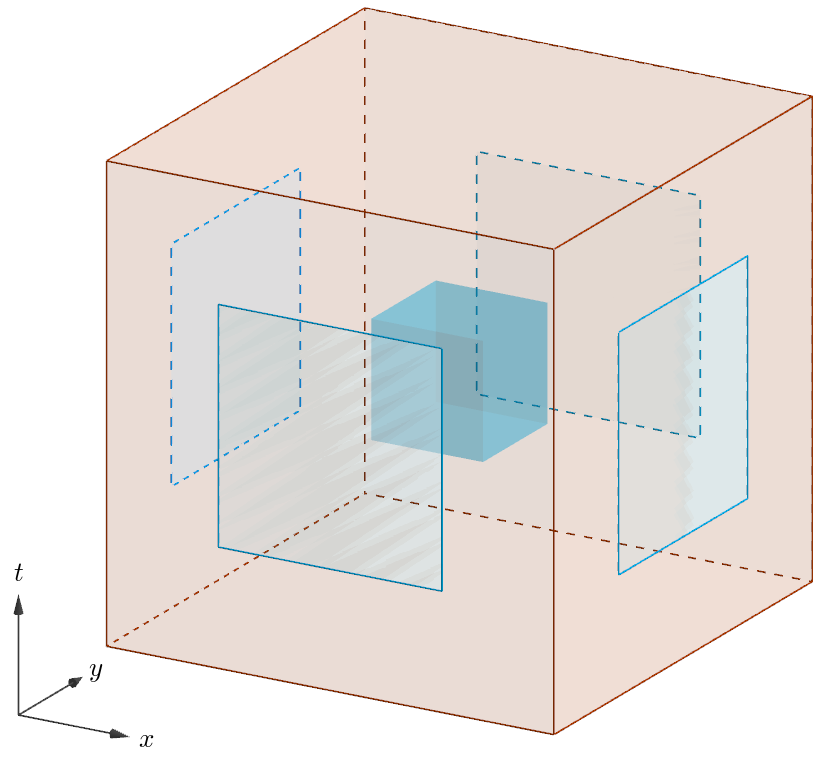
\includegraphics[width=0.7\textwidth]{flux3D.png}
  \caption{Support for $\hat f$}
  \label{fig:flux3D}
\end{figure}

Finally, we need to discuss the test functions. $v$ will basically just be a
combination of $u$ and $\hat u$ as shown in Figure~\ref{fig:v3D} just as
$\bftau$ will be the combination of $\bfsigma$ and $\hat f$ shown in
Figure~\ref{fig:tau3D}.

\begin{figure}[p]
  \centering
  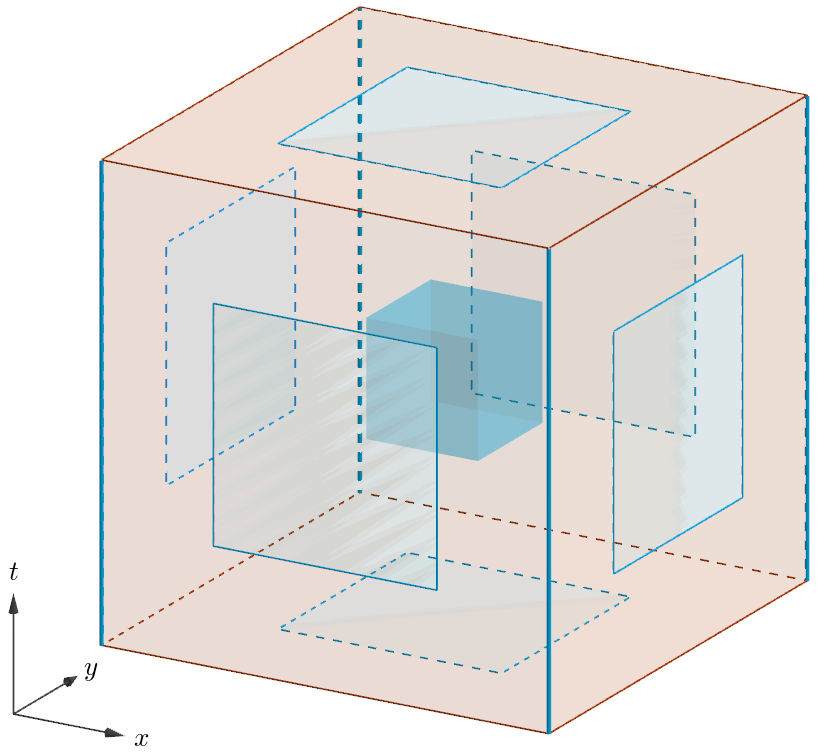
\includegraphics[width=0.7\textwidth]{v3D.png}
  \caption{Support for $v$}
  \label{fig:v3D}
\end{figure}

\begin{figure}[p]
  \centering
  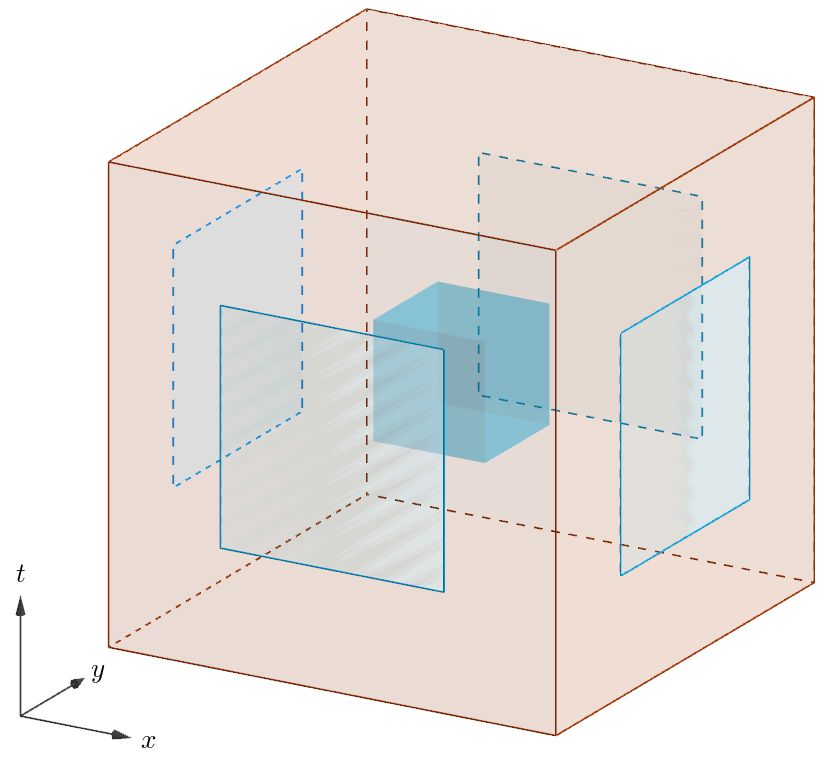
\includegraphics[width=0.7\textwidth]{tau3D.png}
  \caption{Support for $\bftau$}
  \label{fig:tau3D}
\end{figure}

\section*{Practical Aspects}
Now we return to the first order system from Equation~\ref{eq:firstOrderSystem}.
Multiplying by test functions $\bftau$ and $v$, and integrating by parts we
get the bilinear form
\begin{align*}
-\LRp{u,\frac{\partial v}{\partial t}}
+\LRa{\hat u,v\cdot n_t}
+\LRp{\bfsigma,\Grad v}
-\LRa{\widehat{\bfsigma\cdot\mathbf{n_x}}, v}\\
+\LRp{\frac{1}{\epsilon}\bfsigma,\bftau}
+\LRp{u,\Div\bftau}
-\LRa{\hat u,\bftau\cdot\mathbf{n_x}}
=\LRp{f,v}
\end{align*}
where $\widehat{\bfsigma\cdot\mathbf{n_x}}\equiv\hat f$.

Let's examine these terms one at a time. Clearly, volume terms 1, 3, 5, and 6
are just as they are for pure spatial DPG with the exception that vector
quantities are of the dimension of the spatial dimension only. Term 2 will
degenerate on constant space (as a function of time) boundaries, but
we probably don't need any special logic to handle this, because at times
non-constant-time interfaces will have nonzero $n_t$ components (though this
will probably only happen with moving interfaces).
Terms 4 and 7 will degenerate on constant-time (as a function of
space) boundaries. We will probably want to treat constant-time interfaces
uniquely and not even attempt to integrate these terms because they are not
well defined there.

\subsection*{Relationship to H(curl)}

\clearpage

\end{document}
